\documentclass{article}
\usepackage[utf8]{inputenc}
\usepackage[croatian]{babel}
\usepackage[T1]{fontenc}
\usepackage{lmodern}
\usepackage{algorithmic}
\usepackage{algorithm}
\usepackage{longtable}
\usepackage{graphicx}
\usepackage{booktabs}
\usepackage{hyperref}
% Da bi se promjenio stil citiranja umjesto:
% [authoryear, round]
% staviti:
% [numbers, square]
\usepackage[authoryear, round]{natbib}
\usepackage{amsmath}
\usepackage{subfig}
\usepackage{fixltx2e}
\usepackage{todo}
\usepackage{url}
\usepackage{textcomp}

\newcommand{\engl}[1]{(engl.~\emph{#1})}

\begin{document}
\title{Izlučivanje značajki lica Gaborovim filterom}
\author{Tomislav Reicher \and Krešimir Antolić \and Igor Belša \and Marko Ivanković \and Ivan Krišto \and Maja Legac \and Tomislav Novak}

\maketitle

\tableofcontents

\section{Uvod}
Raspoznavanje uzoraka je znanstvena disciplina iz područja računarskih znanosti
čiji je cilj klasifikacija ili razvrstavanje objekata u jedan od brojnih razreda
ili klasa. Iako su područja uporabe brojna u ovom radu koncentacija je na
raspoznavanju vizulanih uzoraka. Točnije, radi se o raspoznavanju lica.

Raspoznavanje lica uključuje računalno prepoznavanje indentiteta na temelju
značajki dobivenih obradom slika lica. Iako ljudima lak zadatak, prepoznavanje
lica i njihova klasifikacija je veoma zahtjevan posao za računalo. Zadatak
postaje tim zahtjevniji ako su lica slikana pod različitim osvijetljenjem,
različitim kutovima ili ako osobe na slikama nemaju uvijek isti izraz lica.

Kao osnovna motivacija za korištenje Gaborovog filtera za izvlačenje značajki je
veza sa biološkim osobinama vida kod sisavaca čiji su receptori osjetljivi na
orijentaciju te imaju karakteristične prostorne frekvencije. Gaborov filter može
iskoristit vizualne osobine kao što su lokalizacija prostora, selekcija
orijentacije i karakteristike prostorne frekvencije
\citep{bhuiyan2007onfacerecognition}\nocite{daugman1985uncertainty}.

% Ovo je opis o čemu koji odjeljak govori. Ovo se MORA nalaziti na kraju uvoda.
U 2.~odjeljku prikazan je matematički model dvodimenzionalnog Gaborovog filtra,
3.~odjeljak navodi objašnjenja pojedinih parametara i njihov utjecaj na krajnji rezultat, 
u 4.~odjeljku objašnjen je način izvlačenja značajki, 
u 5. odjeljku su opisani daljni koraci u raspoznavanju lica, a zaključak je dan u 6.~odjeljku.

\section{Dizajn Gaborovog filtera}
Dvodimenzionalna Gaborova funkcija dana je kao \citep{petkovgabor}:
\begin{equation}
% g(x,y)=\frac{1}{2\pi \sigma^2_{xy}}e^{-\left ( \frac{x'^2 +
% y'^2}{2\sigma^2_{x,y}} \right)} \times \left ( e^{2\pi i r_0 x'} -
% e^{-\frac{r_0^2}{2\sigma^2_{uv}}}\right),
g_{\lambda,\theta,\varphi,\sigma,\gamma}(x,y) = \exp\left ( -
\frac{x'^2+\gamma^2 y'^2}{2\sigma^2}\right ) \cos \left ( 2\pi \frac{x'}{\lambda} + \varphi \right ),
\label{2d-gabor}
\end{equation}
pri čemu su
\begin{eqnarray*}
x' = x \cos \theta + y \sin \theta, \\
y' = -x \sin \theta + y \cos \theta.
\end{eqnarray*}
% gdje je $\sigma_{xy}$ standardna devijacija Gaussove omotnice\TODO{\emph{Gaussian
% envelope}?}koja karakterizira prostorni obujam i širinu filtera.
Frekvencija i odabir orijentacije Gaborovog filtra su izražajnije u domeni
frekvencijskog prikaza predstavljenog Gaborovom funkcijom (\ref{gabor-frek}) koja
određuje koliko filter utječe na svaku frekvencijsku komponentu ulazne slike.
\begin{equation}
G(u,v) = \exp \left ( - \frac{(u-u_0)^2 + (v-v_0)^2}{2\sigma^2_{uv}}\right ) -
\exp \left ( - \frac{r_0^2}{2\sigma^2_{uv}} \right),
\label{gabor-frek}
\end{equation}
\begin{equation}
\sigma_{uv} = \frac{1}{2\pi \sigma_{xy}}.
\end{equation}
Parametri ($u_0$, $v_0$) definiraju prostornu frekvenciju sinusoidalnog vala u
ravnini koji također može biti izražen polarnim koordinatama kao radialna frekvencija $r_0$ i
orijentacija $\theta$:
\begin{eqnarray}
r_0^2 = u_0^2 + v_0^2, \\
\tan \theta = \frac{v_0}{u_0}.
\end{eqnarray}
Osobina Gaborovog filtera definirana je radijalnom frekvencijom $r_0$,
orijentacijom i širinom filtera.

Ako je svrha filtera izvlačenje značajki lica, zanimaju nas četiri orijentacije
\citep{huang2005robust}:
\begin{equation}
\theta_k = \frac{\pi(k-1)}{4},\: k = 1,2,3,4.
\label{equ:orijentacije}
\end{equation}
Orijentacije se odnose na oblu konturu lica, oči i usta koji se nalaze u skoro
horizontalnoj ravnini, te nos koji je u vertikalnoj ravnini.

\section{Utjecaj pojedinih parametara}
Gaborov filter definiraju valna duljina ($\lambda$),
orijentacija ($\theta$), fazni pomak ($\varphi$), omjer dimenzija \engl{aspect ratio}
($\gamma $) i širina filtera \engl{bandwidth} ($b$) \citep{petkovgabor}.

\subsection{Valna duljina ($\lambda$)}
Valna duljina se odnosi na valnu duljinu kosinusa u Gaborovoj funkciji kojom se ujedino definira
i prostorna frekvencija na koju će sam Gaborov filter biti osjetljiv.
Vrijednost valne duljine realan je broj veći ili jednak $2$ koji predstavlja broj slikovnih elemenata (engl. Pixel).

Slike Gaborovih filtera uz parametre $\varphi, \theta = 0,\: b = 1$, i $\gamma =
0.5$ možete vidjeti na slici \ref{fig:filter-wavelengths}.

\begin{figure}[htb]
\centering
\subfloat[Filter uz $\lambda = 5$.]{
\label{fig:filter-lambda-5}

\includegraphics[width=4cm]{images/wavelength5.jpg}
}
\hspace{50pt}
\subfloat[Filter uz $\lambda = 10$.]{
\label{fig:filter-lambda-10}

\includegraphics[width=4cm]{images/wavelength10.jpg}
}
\caption{Gaborov filter uz različite valne duljine.}
\label{fig:filter-wavelengths}
\end{figure}

% TODO: Pogledati o čemu se ovdje radi\ldots Gledao sam formulu, ništa pametno
% nisam zaključio, generirao sam slike, također ništa pametno\ldots Nešto mi
% promiče\ldots Zakomentirao sam tu rečenicu dok mi ne postane smislena.
%Uz $\lambda = 2$, ne bi se smjela koristiti kombinacija $\varphi = \pm 90$ jer
%u tom slučaju Gaborova funkcija je uzrokovana u svojim
%nul--prijelazima\TODO{``sampled in its zero crossings''?}.
Da bi se spriječila pojava neželjenih efekata na rubovima slike prilikom filtriranja slike Gaborovim filtrom, vrijednost valne
duljine mora biti manja od $\frac{1}{5}$ veličine slike koja prolazi kroz
filter. Filter sa prevelikom valnom duljinom može se vidjeti na slici
\ref{fig:wavelength-overflow}. U danom primjeru filter djeluje na području
širine 100 piksela, a filter je širok 30 piksela.

\begin{figure}[htb]
\begin{center}

\includegraphics[width=4cm]{images/wavelength30overflow.jpg}
\end{center}
\caption{Prikaz filtera uz preveliku valnu duljinu.}
\label{fig:wavelength-overflow}
\end{figure}

\subsection{Orijentacija ($\theta$)}
Orijentacija određuje kut između normale i paralelnih pruga Gaborovog
filtera odnosno kut između normale i smjera rasprostiranja moduliranog sinusnog signala.
Određena je kutom od $0$ do $360$ stupnjeva. Prikaze Gaborovog filtera sa
orijentacijama od 45\textdegree, 80\textdegree\,i 0\textdegree\, možete vidjeti
na slikama \ref{fig:filter-orientation-45}, \ref{fig:filter-orientation-80} i
\ref{fig:filter-lambda-10}.


\begin{figure}[htb]
\centering
\subfloat[Filter uz $\theta = 45$\textdegree.]{
\label{fig:filter-orientation-45}

\includegraphics[width=4cm]{images/orientation45.jpg}
}
\hspace{50pt}
\subfloat[Filter uz $\theta = 80$\textdegree.]{
\label{fig:filter-orientation-80}

\includegraphics[width=4cm]{images/orientation80.jpg}
}
\caption{Gaborov filter uz različite orijentacije.}
\label{fig:filter-orientations}
\end{figure}

\subsection{Fazni pomak ($\varphi$)}
Ovaj parametar određuje fazni pomak kosinusa unutar Gaborove funkcije.
Ispravne vrijednosti su realni brojevi između $-180$ i $180$ stupnjeva. Prikaze
Gaborovog filtera sa fazama od 45\textdegree, 180\textdegree\, i 0\textdegree\,
možete vidjeti na slikama \ref{fig:filter-phase-45},
\ref{fig:filter-phase-180} i \ref{fig:filter-lambda-10}.

\begin{figure}[htb]
\centering
\subfloat[Filter uz $\varphi = 45$\textdegree.]{
\label{fig:filter-phase-45}
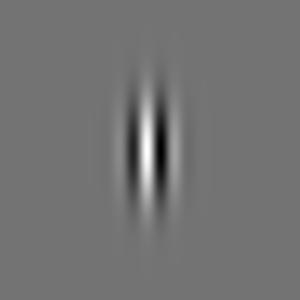
\includegraphics[width=4cm]{images/phase45.jpg}
}
\hspace{50pt}
\subfloat[Filter uz $\varphi = 180$\textdegree.]{
\label{fig:filter-phase-180}
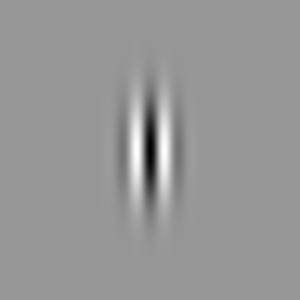
\includegraphics[width=4cm]{images/phase180.jpg}
}
\caption{Gaborov filter uz različite faze.}
\label{fig:filter-phases}
\end{figure}

Vrijednosti $0$\textdegree\, i $180$\textdegree\, odgovaraju
središnje--simetričnim funkcijama, a $-90$\textdegree\, i $90$\textdegree\,
anti--simetričnim funkcijama (primjer filtera se može vidjeti na slici
\ref{fig:phase-90}). Svi ostali slučajevi odgovaraju asimetričnim funkcijama.

\begin{figure}[htb]
\begin{center}
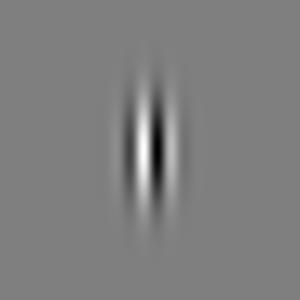
\includegraphics[width=4cm]{images/phase90.jpg}
\end{center}
\caption{Filter uz fazu od 90\textdegree (anti--simetrija).}
\label{fig:phase-90}
\end{figure}

\subsection{Omjer dimenzija ($\gamma $)}
Parametar koji se preciznije naziva prostorni omjer dimenzija, određuje
eliptičnost Gaborove funkcije tj. odnos između devijacija Gaussove funkcije u $x$ i $y$ smjeru. Za $\gamma = 1$ eliptičnost se svodi na krug.
Za $\gamma < 1$ funkcija je izdužena u smjeru paralelnom s paralelnim prugama
funkcije. Primjer filtera sa različitim omjerima
dimenzija se može vidjeti na slici \ref{fig:filter-ratios}.

\begin{figure}[htb]
\centering
\subfloat[Filter uz $\gamma = 0.5$.]{
\label{fig:filter-gamma-05}

\includegraphics[width=4cm]{images/wavelength10.jpg}
}
\hspace{50pt}
\subfloat[Filter uz $\gamma = 1$.]{
\label{fig:filter-gamma-1}

\includegraphics[width=4cm]{images/ratio1.jpg}
}
\caption{Gaborov filter uz različite omjere dimenzija.}
\label{fig:filter-ratios}
\end{figure}

\subsection{Širina filtera ($b$)}
Prostorna širina filtera $b$ Gaborovog filtra je povezana sa
omjerom $\frac{\sigma}{\lambda}$, pri čemu su $\sigma$ i $\lambda$ standardna
devijacija Gaussove funkcije i valna duljina kosinusa. Prostorna širina definirana je
s:
\begin{eqnarray}
b = \log_2{\left ( \frac{\frac{\sigma}{\lambda}\pi + \sqrt{\frac{\ln2}{2}}}
{\frac{\sigma}{\lambda}\pi - \sqrt{\frac{\ln2}{2}}} \right )}, \\
\frac{\sigma}{\lambda} =
\frac{1}{\pi}\sqrt{\frac{ln2}{2}}\cdot\frac{2^b+1}{2^b-1}.
\end{eqnarray}
Prilikom izvedbe filtra vrijednost $\sigma$ se ne može direktno odrediti. Ona se može mijenjati samo
preko vrijednosti širine filtera, $b$.

Širina filtera se određuje kao realni pozitivni broj. Što je širina manja,
$\sigma$ je veća i povećava se broj naglašavajućih i prigušavajućih pruga
Gaborovog filtera.~ Primjere filtera sa
različitim širinama možete vidjeti na slikama \ref{fig:filter-bandwidth-05} i
\ref{fig:filter-bandwidth-2}. Na prethodnim primjerima korištena je širina
filtera od $b = 1$.

\begin{figure}[htb]
\centering
\subfloat[Filter uz $b = 0.5$.]{
\label{fig:filter-bandwidth-05}
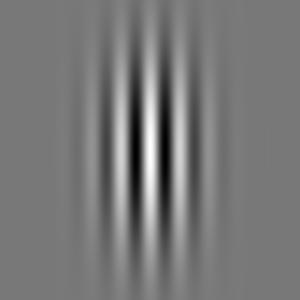
\includegraphics[width=4cm]{images/bandwidth05.jpg}
}
\hspace{50pt}
\subfloat[Filter uz $b = 2$.]{
\label{fig:filter-bandwidth-2}

\includegraphics[width=4cm]{images/bandwidth2.jpg}
}
\caption{Gaborov filter uz različite širine.}
\label{fig:filter-bandwidths}
\end{figure}

\section{Izvlačenje značajki pomoću gaborovog filtera}
Osnovna ideja korištenja Gaborovog filtra pri raspoznavanju je filtriranje početne 
slike filtrom s ciljem izlučivanja značajki za kasniju klasifikaciju.
Odziv Gaborovog filtra osjetljiv je na lokalnu prostornu frekvenciju i odgovarajuću orijentaciju
ulaznog signala, odnosno slike, pa pod pretpostavkom da su Gaborovim filtrom izlučene
odgovarajuće frekvencije i orijentacije moguće je raspoznavati različite osobe
temeljem slika njihovih lica.

Izlaz Gaborovog filtra dobiva se konvolucijom klizečeg prozora slike i Gaborove
funkcije.

Neka je $I(x,y)$ slika. Konvolucija slike $I(x,y)$ i Gaborove funkcije dana je
sa:
\begin{equation}
O(x,y,r_0, \theta_k) = I(x,y) * g(x,y,r_0, \theta_k),
\label{konvolucija-filter-slika}
\end{equation}
pri čemu je $k = 1, 2, 3, 4$. $O(x,y,r_0, \theta_k)$ nazivamo Gaborov prikaz
slike $I(x,y)$.

Rezultantna funkcija je kompleksna funkcija s realnim i imaginarnim dijelom. Prilikom 
filtriranja ulazne slike Gaborovim filtrima različitih frekvencija i orijentacije nastaje
skup kompleksnih funkcija koje se tada grupiraju u odgovarajući vektor značajki.
Vektor značajki nije nužno ograničen na prikaz pomoću kompleksnih brojeva te ga je moguće
prikazati i kao vektor amplituda odnosno vektora faza rezultantnih funkcija nastalih filtiranjem.
Kvaliteta izlučenih značajki ovisi iznimno o parametrima Gaborovog filtera te je 
naš zadatak u ovom radu je pronaći optimalne parametre Gaborovog filtra za izlučivanje
značajki ljudskog lica.


\section{Klasifikacija}

Nakon izlučivanja značajki Gaborovim filtrom dobiven je vektor značajki koji se koristi za klasifikaciju. 
Kako je dobiveni vektor visoke dimenzionalnosti potrebno je izvršiti redukciju prostora značajki na nižedimenzionalan prostor.
Neke od metoda koje se pritom koriste su linearna diskriminanta analiza (engl. Linear Discriminant Analysis) i analiza glavnih komponenti
(engl. Principal Component Analysis). 
Za klasifikaciju vektora značajki dostupno je mnogo različitih klasifikatora poput neuralnih mreža, stroja s potpornim vektorima i sl.
te će se u okviru ovog rada ispitati učinkovitost različitih metoda klasifikacije kako bi se pronašla ona s najvećom uspješnošću.

\section{Zaključak}

Korištenje Gaborovog filtra ima dobru podlogu u biološkim osnovama vida
sisavaca te se očekuje da će se njegovom upotrebom, korištenjem različitih klasifikatora i
automatiziranom optimizacijom parametara postići uspjeh u raspoznavanju lica različitih osoba.

\bibliography{literatura}
\bibliographystyle{plainnat}

\end{document}
